\setchapterpreamble[u]{\optmargintoc}
\chapter{Background}
\labch{background}

\section{Hydrodynamics}

At the length scales of cilia (generally between one and a few tens of micrometres \sidecite{saggese_development_2012}) fluid flow looks very different to what is seen at a human scale. For a human in a swimming pool, inertial forces are hugely important, allowing a competent swimmer to glide several metres on a single stroke. A bacterium in a puddle of water sees a very different world, where the environment is dominated by viscous forces; if a swimming bacterium were to stop actively propelling itself, it would only coast approximately $10\,\mathrm{pm}$ (slightly less than the diameter of a hydrogen atom), and come to a halt in under a microsecond~\sidecite{purcell_life_1977}, as the friction is so much more important than the bacterium's minuscule momentum. Despite this, the swiftest bacteria can swim at hundreds of body lengths per second~\sidecite{zhang_swimming_2014}.

This dominance of viscous forces over inertia is quantified by the dimensionless Reynolds number, defined as
\begin{equation}
    \mathrm{Re} = \frac{L u \rho}{\mu},
\end{equation}
where $L$ is the length scale, $u$ is the speed of motion, $\rho$ is the fluid density, and $\mu$ is the dynamic viscosity of the fluid.
% (not to be confused with the similarly named \textit{kinematic} viscosity, which is usually given the symbol $\nu$ and defined as $\nu\equiv\mu/\rho$)
Plugging in reasonable numbers, we find that for a cilium or bacterium, the Reynolds number is around $\sim 10^{-5} - 10^{-4}$, which, being much less than one, tells us that inertial forces are tiny enough to be entirely negligible compared to fluid viscosity. For comparison, a human in a swimming pool experiences a Reynolds number of $\sim 10^3 - 10^4$, around a hundred million times greater than the cilium. For a human to experience this same viscous dominance that a cilium feels, they would have to swim at their normal swimming speed, but in a fluid around $10 - 100$ times more viscous than even the thickest peanut butter~\sidecite{citerne_rheological_2001}.

\subsection{Stokes flow}

The Navier-Stokes equation for an incompressible fluid, describing the velocity $\mathbf{u}$ and pressure $p$ of a fluid experiencing an external force per unit volume $\mathbf{f}$, can be written as
\begin{equation}
    \rho \left( \frac{\partial \mathbf{u}}{\partial t} + \left( \mathbf{u} \cdot \nabla \right) \mathbf{u} \right) = -\nabla p + \mu \nabla^2 \mathbf{u} + \mathbf{f}.
\end{equation}
This equation is nonlinear and famously hard to solve\boxedsidenote{The proof of the existence of a smooth and globally defined solution to the Navier-Stokes equations is one of the Millennium Prize Problems. Anyone who is able to prove such a solution exists in every case will receive a prize of \$1,000,000.}. However, as previously mentioned, inertia is negligible at the scale of cilia. Many of the terms in this equation represent inertial forces that are not relevant, so we can simplify this equation heavily to obtain the Stokes equation:
\begin{align}
    \mu\nabla^2\mathbf{u}-\nabla p +\mathbf{f} &= 0,\\
    \nabla\cdot \mathbf{u} &= 0.
\end{align}
This equation has no explicit time dependence, which means that a change in the force $\mathbf{f}$ or boundary conditions propagates instantly to the fluid, but if the force and boundary conditions are unchanged, the flow field $\mathbf{u}$ is constant in time. The form of the equations also ensures that if $\mathbf{u}$ is a solution for a given $\mathbf{f}$, then so is $\mathbf{-u}$ for $\mathbf{-f}$; the equations are `reversible'. This leads to an interesting consequence known as Purcell's scallop theorem: at low Reynolds number, any series of actions followed by the reverse of those actions can't generate a net motion. The organism that gives the theorem its name, the scallop, swims by opening and closing its shell, and is therefore unable to swim in a Stokes fluid~\sidecite{purcell_life_1977}. For motile cilia, this lesson is of the utmost importance: if fluid is to be pumped, waving back and forth in a plane without bending is insufficient. The motion needs to be cyclic, but not reversible. % Ugh I really wish I could bring up the ciliary beat here

\subsection{Solving the Stokes equations}\label{subsec:solvingstokes}

Computing the flow due to a moving cilium is complicated, and in practice requires some simplifying assumptions that change depending on the context and what kind of accuracy is needed. The simplest possible solution to the Stokes equations is the Stokeslet, which represents the fluid flow a displacement $\mathbf{r}$ from a point force $\mathbf{F}$:
\begin{align}
    \mathbf{u(\mathbf{r})} &= \mathcal{S}(\mathbf{r}) \cdot \mathbf{F} \\
    &\equiv \frac{1}{8\pi\mu} \left( \frac{\mathbb{1}}{\left| \mathbf{r} \right|} + \frac{\mathbf{rr}}{\left| \mathbf{r} \right|^3} \right) \cdot \mathbf{F},\nonumber
\end{align}
under the assumption that the flow speed and pressure decays to zero infinitely far away. However, this is a very poor approximation of a cilium, and would almost never be a sufficiently good simplification for practical purposes. 

For a start, the cilium is found on the surface of a cell, which means that one has to account for the effect of the cell on the fluid flow. Generally, the best boundary condition to use in this case is the no-slip condition, wherein the fluid flow relative to the cell's surface is stationary. This has fairly significant experimental backing for fluids where viscosity dominates over inertia~\sidecite{day_no-slip_1990}, so we will adopt it here as well. 

To compute the flow due to a point force in the presence of a no-slip boundary, we can use a solution sometimes called the Blakelet~\sidecite{blake_note_1971}. In much the same way that it is possible to find the electric field due to a charged particle in the presence of a conducting boundary by introducing a second imaginary `image' particle with the opposite charge reflected in the conducting boundary, Blake realised it was possible to model the flow due to a Stokeslet in the presence of a no-slip boundary by creating an `image system', consisting of multiple flow singularities (one of which is a Stokeslet with equal magnitude and opposite direction), located where the mirror image of the real particle would be: see Fig.~\ref{fig:blake_image_system} for a diagram of the image system. The derivation is complicated, and the full treatment can be found in \etalcite{blake_note_1971}, but the result is incredibly useful for modelling the hydrodynamics of cilia: if we have a point force in a fluid at a position $(r_1, r_2, h)$ above a no-slip boundary, we also introduce an `image particle' which is reflected in the $z=0$ axis from the real particle. In other words, the image will be located at $(r_1, r_2, -h)$. We denote the displacement from the image particle to the position where we are interested in the fluid flow as $\mathbf{R}$, and thus the Blakelet can be written as:
\begin{align}
    u_j&(\mathbf{r}, \mathbf{R}) = \mathcal{B}_{jk} F_k \nonumber \\ 
    &= \frac{1}{8\pi\mu} \left[ \left( \frac{1}{r} - \frac{1}{R} \right) \delta_{jk} + \frac{r_j r_k}{r^3} - \frac{R_j R_k}{R^3} \right.\label{eq:blake} \\
    &+ \left. 2h\left( \delta_{k\alpha}\delta_{\alpha \beta} - \delta_{k3}\delta_{3\beta} \right) \frac{\partial}{\partial R_\beta} \left( \frac{h R_j}{R^3} - \left\{ \frac{\delta_{j3}}{R} + \frac{R_j R_3}{R^3} \right\} \right) \right] \cdot F_k.\nonumber
\end{align}
Note the use of Einstein summation notation, meaning that repeated indices are summed over\boxedsidenote[][-70pt]{In the same notation, the Stokeslet would become: \begin{align*}u_j(\mathbf{r}) &= \mathcal{S}_{jk} F_k \\
&= \frac{1}{8\pi\mu} \left( \frac{\delta_{jk}}{r} + \frac{r_j r_k}{r^3} \right) F_k.\end{align*}}, i.e. $r_i r_i = r_1^2 + r_2^2 + \dots = r^2$. 

\begin{figure}
    \centering
    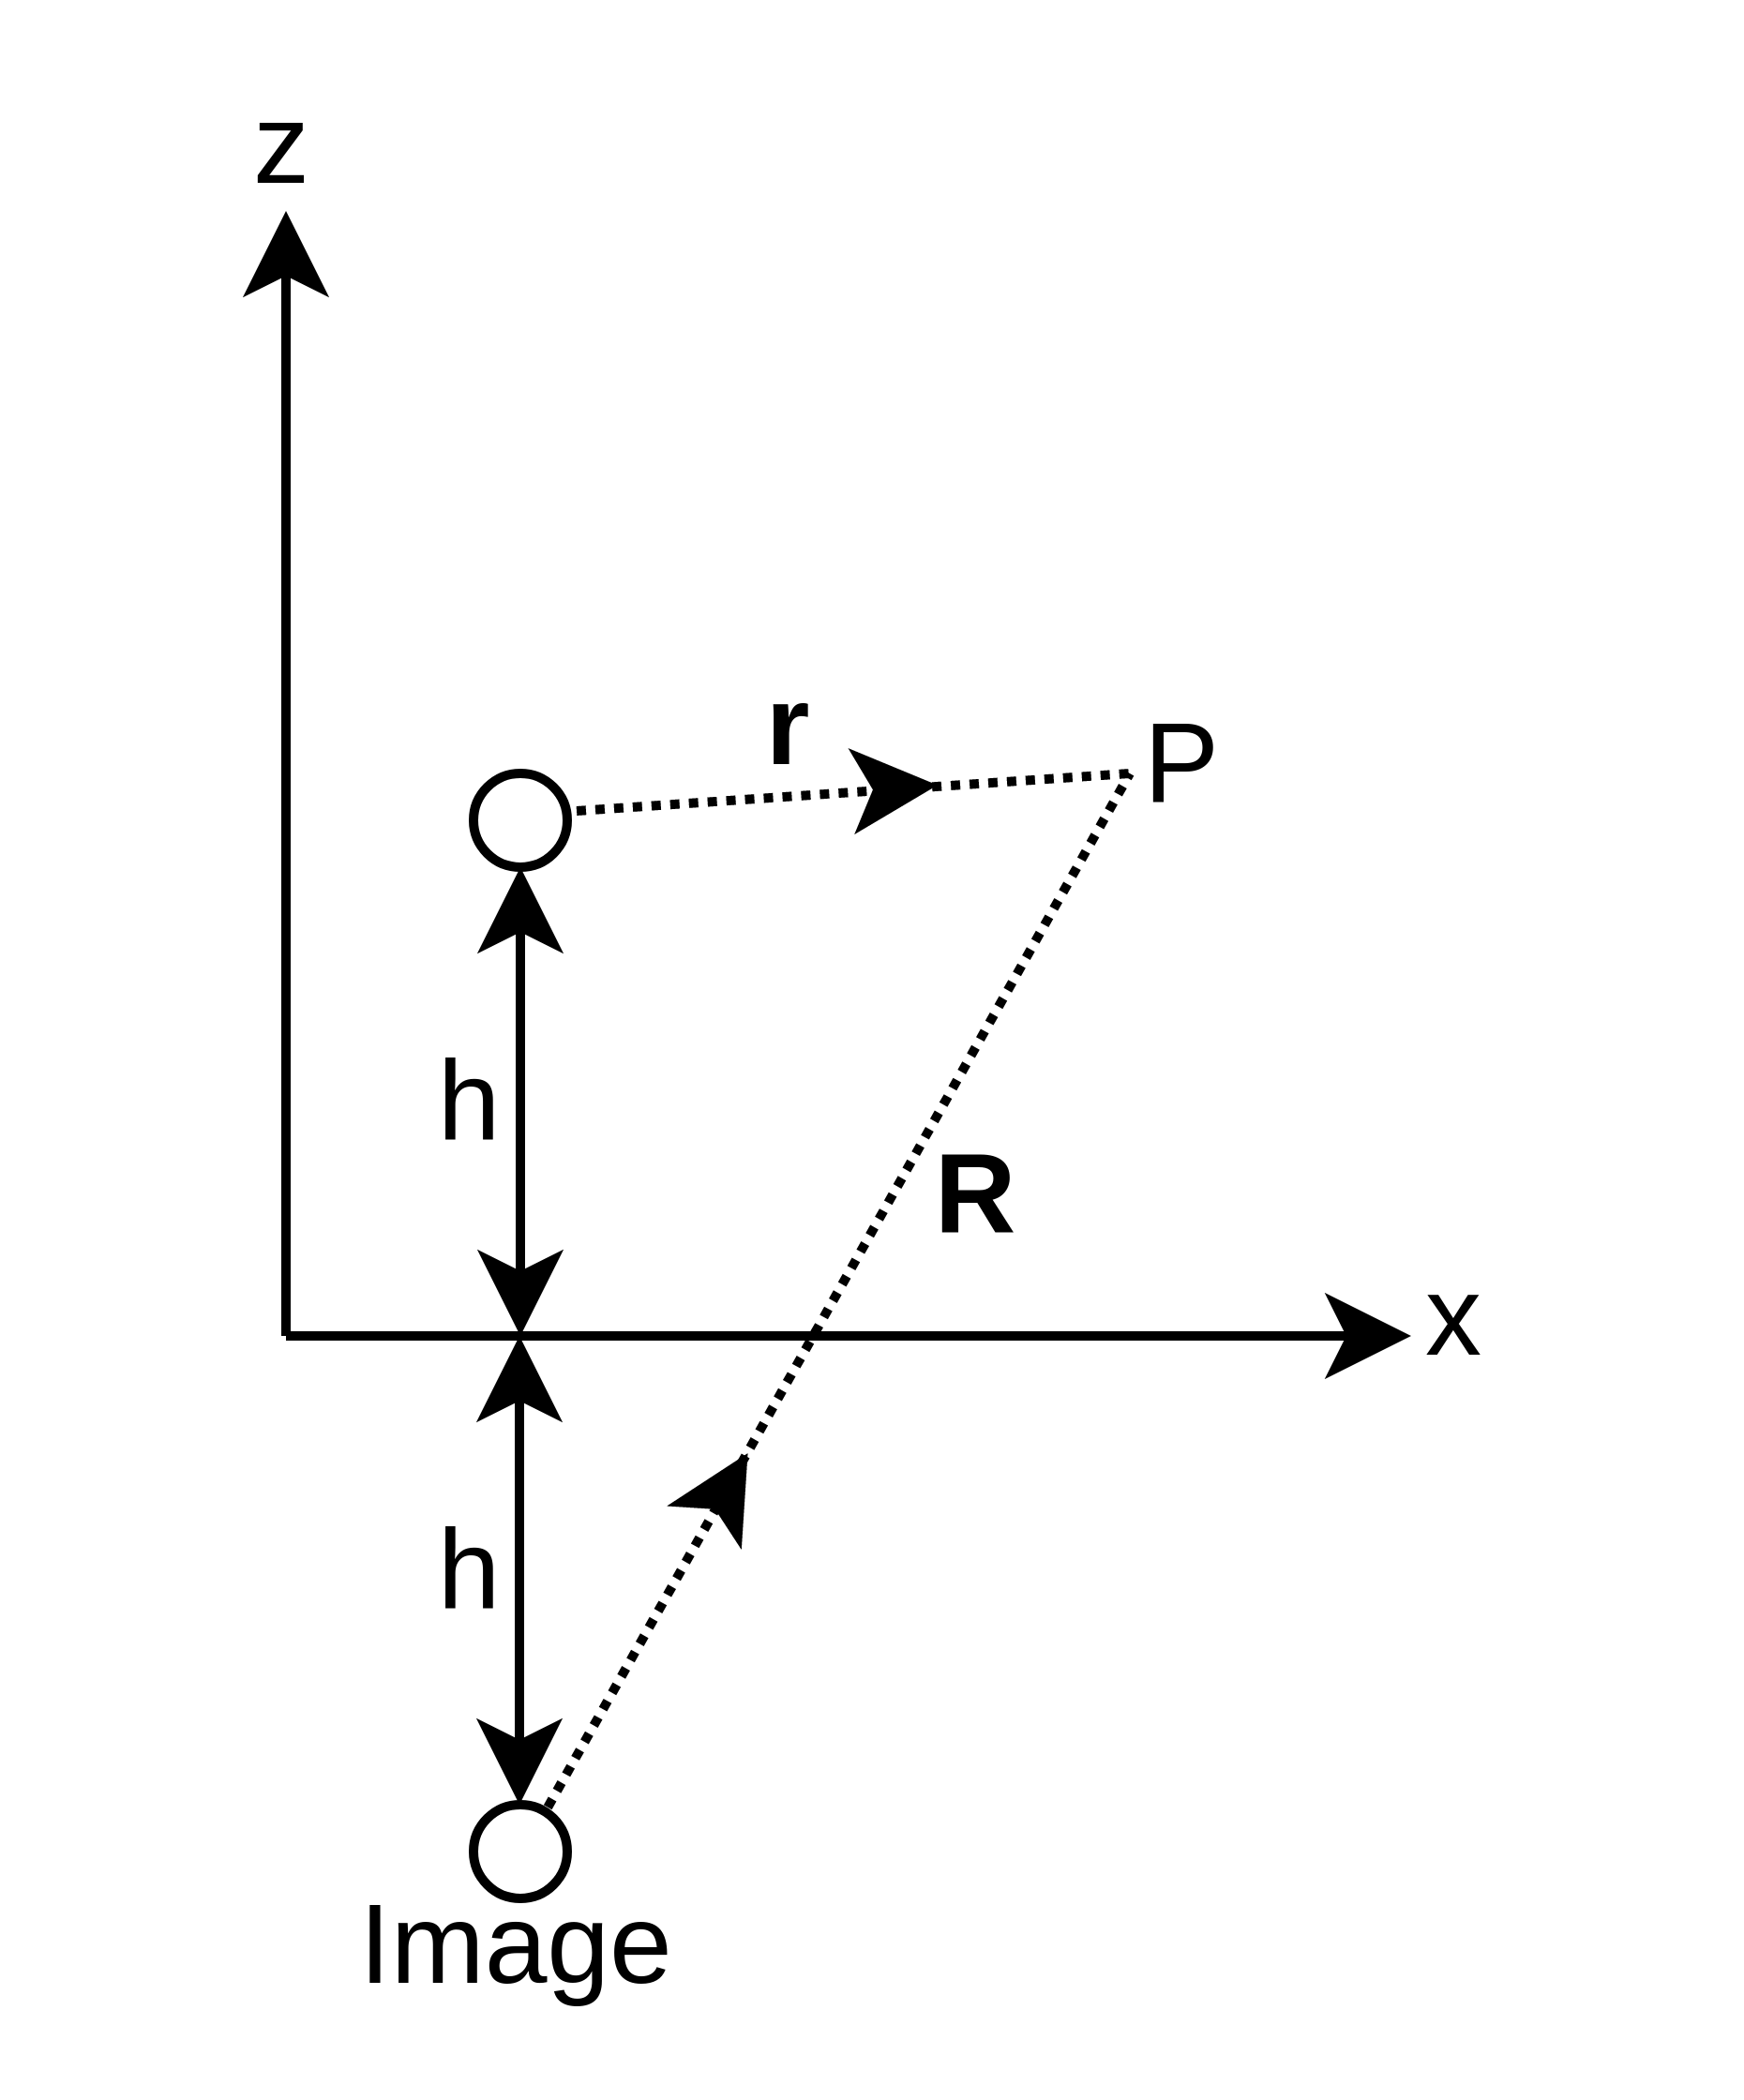
\includegraphics[width=0.7\textwidth]{images_other/blake_reproduction.png}
    \caption{The image system that underpins the Blake tensor. The real Stokeslet is a distance $h$ above the no-slip boundary at $z=0$, and the image system is found a distance $h$ below the boundary. $P$ is the observation point at which we want to compute the flow.}
    \label{fig:blake_image_system}
\end{figure}

This can be rewritten as a Stokeslet plus an `image' contribution:
\begin{equation}
    u_j(\mathbf{r}, \mathbf{R}) = (\mathcal{S}_{jk} + \mathcal{B}^\text{im}_{jk}) F_k.
\end{equation}
The image contribution decays to zero if the particle is far enough from the boundary.

\begin{figure}
    \captionsetup[subfigure]{format=subcap}
    \centering
    \begin{subfigure}[t]{0.45\linewidth}
        \centering%
        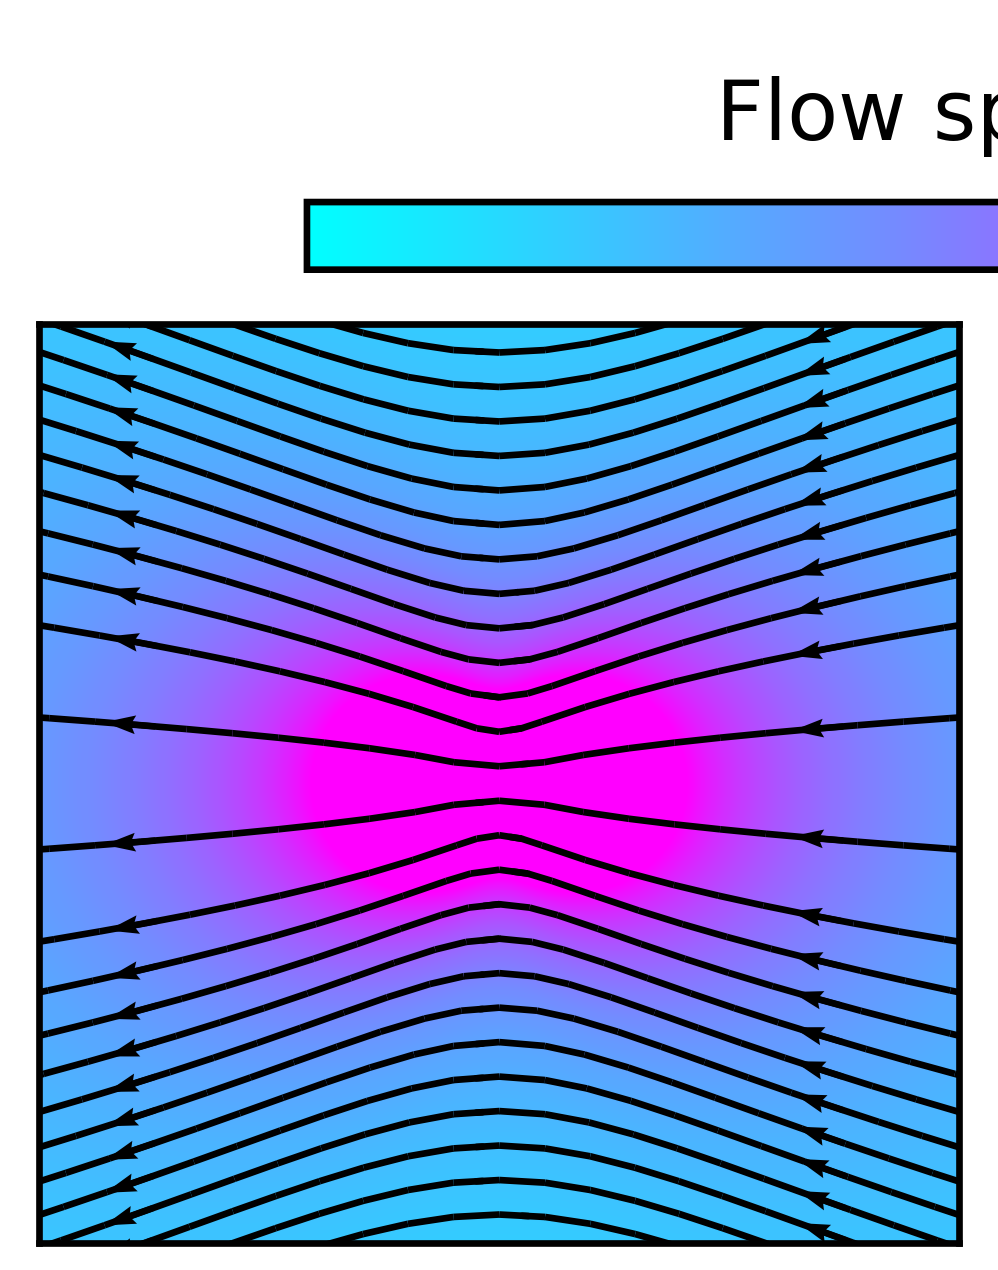
\includegraphics[width=\textwidth]{images_other/stokes_flow_left.png}%
        \caption{Stokes flow due to a moving Stokeslet}%
        \label{fig:flow_sphere_blake}%
    \end{subfigure}%
    \hspace{-20000sp}%
    \begin{subfigure}[t]{0.45\linewidth}%
        \centering%
        \raisebox{10000sp}{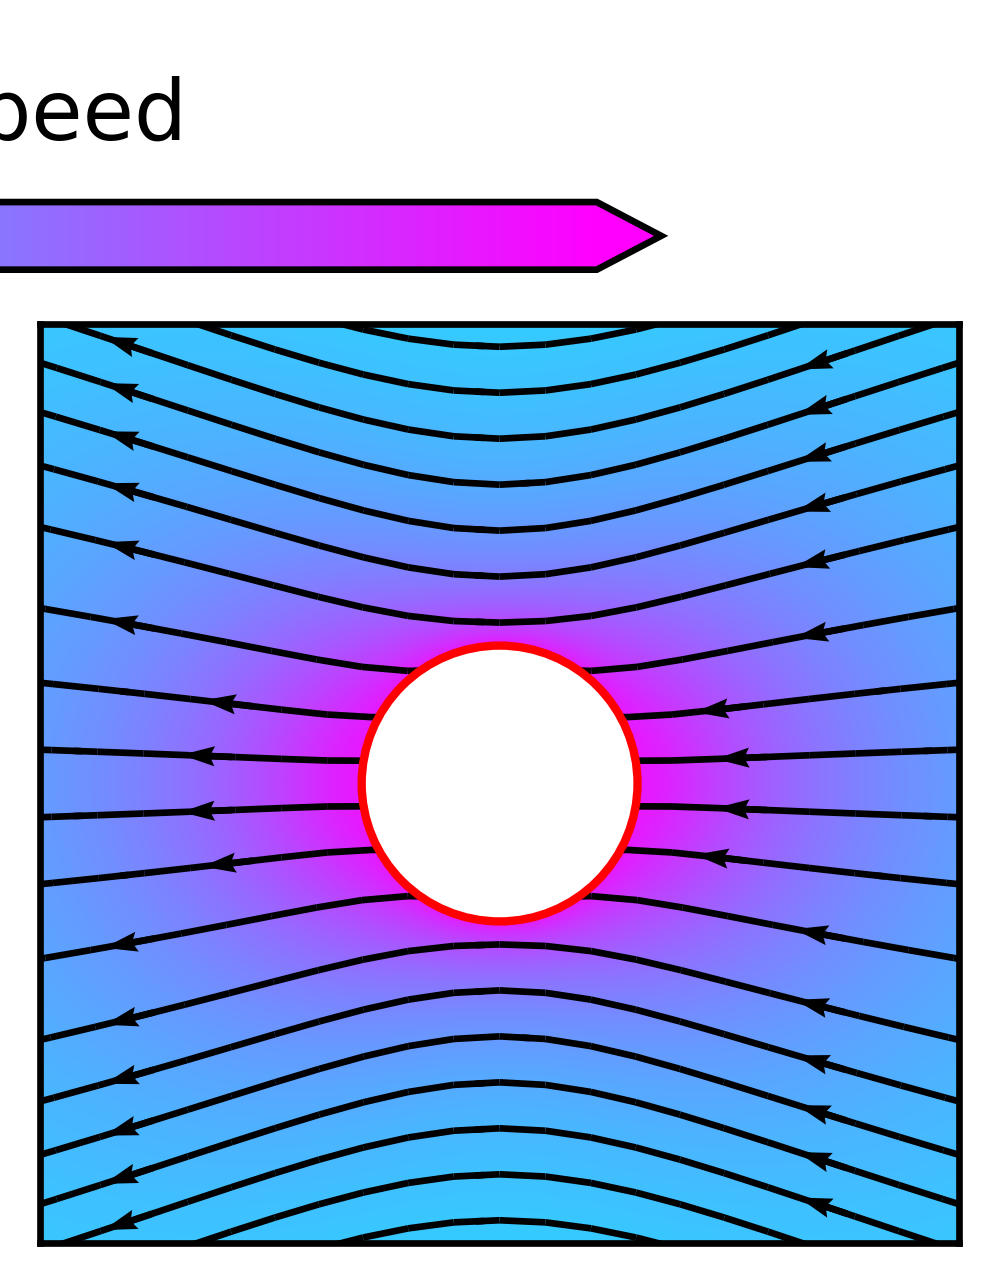
\includegraphics[width=\textwidth]{images_other/stokes_flow_right.png}}%
        \caption{Stokes flow due to a finite-sized sphere}%
        \label{fig:flow_sphere_rp}%
    \end{subfigure}
    
    \begin{subfigure}[t]{0.45\linewidth}
        \centering%
        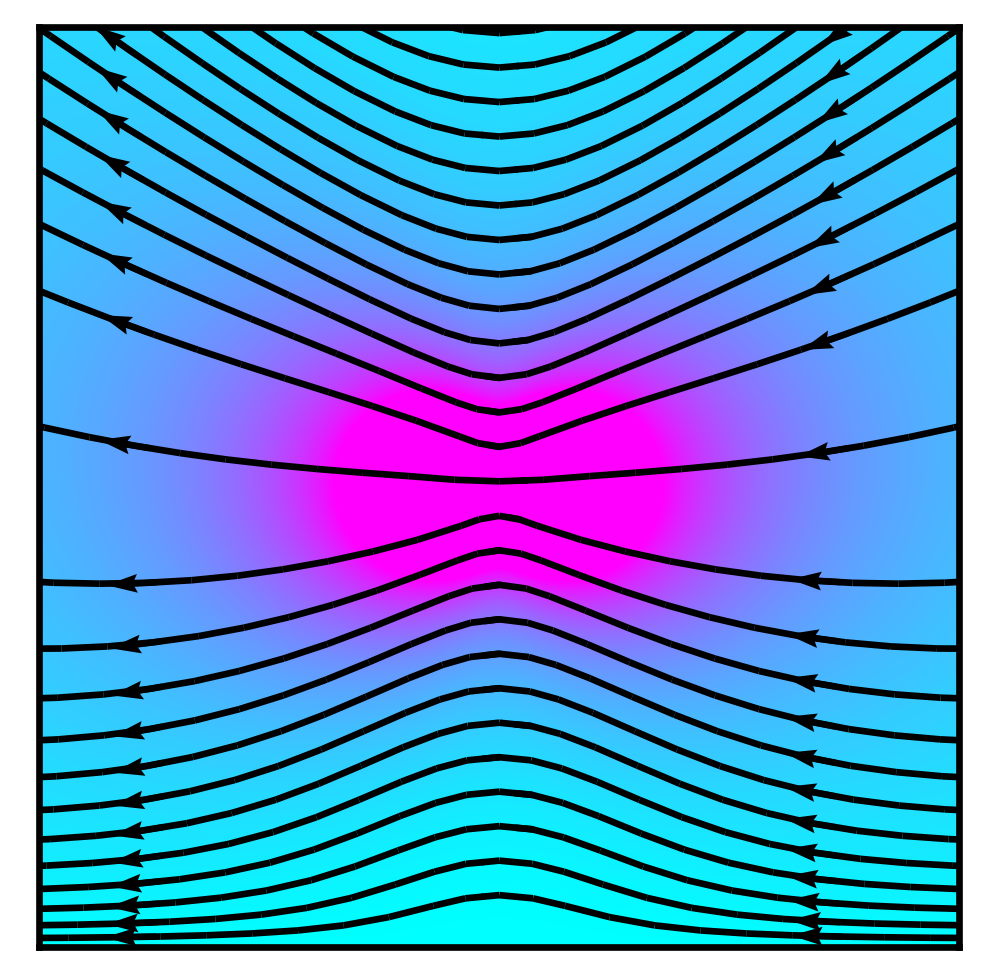
\includegraphics[width=\textwidth]{images_other/stokes_flow_bottomleft.png}%
        \caption{Flow due to a moving Blakelet near a boundary}%
        \label{fig:flow_sphere_blake_bc}%
    \end{subfigure}%
    \hspace{-20000sp}%
    \begin{subfigure}[t]{0.45\linewidth}%
        \centering%
        \raisebox{10000sp}{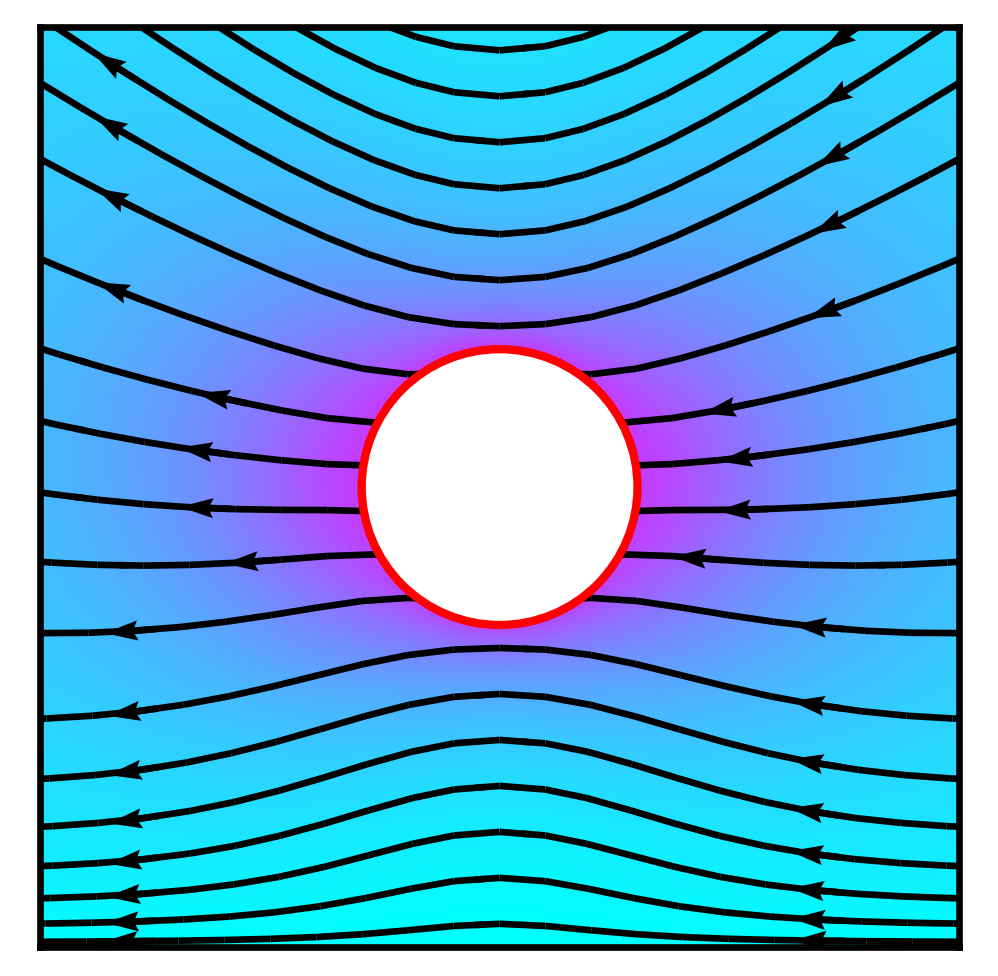
\includegraphics[width=\textwidth]{images_other/stokes_flow_bottomright.png}}%
        \caption{Flow due to a moving finite-sized sphere near a boundary}%
        \label{fig:flow_sphere_rp_bc}%
    \end{subfigure}
    \caption{Different solutions to the Stokes equations corresponding to various Green's functions. (a) and (b) show the flows far away from a boundary, whereas (c) and (d) show the flow field near a no-slip boundary. One can see how the fluid is much slower near the boundary at the bottom edge of the plots, and how the fluid flow is altered.}
    \label{fig:flow_sphere}
\end{figure} % TODO: entire thing in lab frame might make more sense, i.e replace top left and drop top right.

Far away from the cilium, the Blakelet is a very good approximation for the fluid flow due to a moving sphere or even a whole cilium, despite assuming a single point force -- in fact, in the far-field\boxedsidenote[][-100pt]{`Far-field' refers to the fluid behaviour far from the cilium, where only the terms in the force response that decay very slowly with distance are important. `Near-field' refers to the fluid behaviour much closer to the cilium, where the higher order terms are also relevant.} limit, it is exactly the same as the flow due to a sphere acted upon by a force~\sidecite[80pt]{vilfan_generic_2012}. However, closer to the cilium, something more accurate is required; to achieve this, we can integrate the Blakelet over the surface of a sphere of radius $a$ to obtain a version of the Rotne-Prager tensor, modified to include a no-slip boundary. This new mobility satisfies the no-slip boundary on the surface of the sphere. The Rotne-Prager tensor can be written in terms of the Blake tensor as:
\begin{equation}
    \mathcal{M}_{jk} = \left( 1 + \frac{a^2}{6}\nabla^2_{\mathbf{r}_j} \right) \left( 1 + \frac{a^2}{6}\nabla^2_{\mathbf{r}_k} \right) \mathcal{B}(\mathbf{r}_j, \mathbf{r}_k)\label{eq:rp_offdiag}
\end{equation}
for the off-diagonal elements, and
\begin{equation}
    \mathcal{M}_{jj} = \frac{1}{6\pi\mu a}\mathbb{1} + \left( 1 + \frac{a^2}{6}\nabla^2_{\mathbf{r}_j} \right) \left( 1 + \frac{a^2}{6}\nabla^2_{\mathbf{R}_j} \right) \mathcal{B}^\text{im}(\mathbf{r}_j, \mathbf{R}_j)\label{eq:rp_diag}
\end{equation}
for the diagonal elements~\sidecite{gauger_fluid_2009}. The full form of the tensor is much too long to write here, but see for example \etalcite{vilfan_self-assembled_2010}. Some of the fluid flow solutions discussed here are shown in Fig.~\ref{fig:flow_sphere}. Our work in later chapters will make extensive use of this corrected Rotne-Prager tensor.

\FloatBarrier

\nosidecite{gauger_fluid_2009,guazzelli_physical_2011}%\todo{I think we basically neglect F for the offdiagonal terms because it's a higher order contribution; to lower order the sphere is force-free. This doesn't apply to the diagonal case, so we get this eta stuff. But ask Andrej!}
\begin{kaobox}[title=Rotne-Prager derivation]
    The Rotne-Prager tensor can be derived (following~\cite{gauger_fluid_2009}) by integrating the Blakelet over the surface of a sphere of radius $a$ and its centre at $\mathbf{r_s}$:
    \begin{equation}
        \mathbf{u}(\mathbf{r}) = \int_S \mathcal{B}(\mathbf{r}, \mathbf{r}') \mathbf{f}(\mathbf{r}') \, \mathrm{d}S'.
    \end{equation}
    To first order, the force density $\mathbf{f}$ is just the total force $\mathbf{F}$ divided by the surface area of the sphere, which means that we can expand the force and the Blake tensor around $\mathbf{r}'=\mathbf{r}_s$ to get
    \begin{equation}
        \mathbf{u}(\mathbf{r}) \approx \left[ \left( 1 + \frac{a^2}{6} \nabla^2_{\mathbf{r}'} \right) \mathcal{B}(\mathbf{r}, \mathbf{r}') \right]_{\mathbf{r}' = \mathbf{r}_s} \cdot \mathbf{F}.\label{eq:rpderivation1}
    \end{equation}
    Now, Faxén's law tells us that the velocity of a sphere of radius $a$ experiencing a hydrodynamic force $\mathbf{F}$ in a flow is given by:
    \begin{equation}
        \mathbf{F} = 6\pi\mu a \left[ \left( 1 + \frac{a^2}{6}\nabla^2 \right) \mathbf{u}_0 - \mathbf{u}_\text{s} \right]
    \end{equation}
    where $\mathbf{u}_0$ is the fluid flow that would be at the centre of the sphere if the sphere was not there~\cite{guazzelli_physical_2011}, so we can combine this with Eq.~\eqref{eq:rpderivation1}, eliminating $\mathbf{u}(\mathbf{r})=\mathbf{u}_0$ to find the diagonal and off-diagonal terms of the Rotne-Prager tensor.
\end{kaobox}

\subsection{Modelling the motile cilium}

% \todo{Give a brief overview here: you've got your RFT, SBT, regularised stokeslet, and FEM/BEM. You could afford to spend a paragraph talking about each, then say why you're opting for RPY.}

Slender bodies are of great interest in a lot of fields, especially within biophysics: cilia and the superficially similar bacterial flagella are used for swimming and pumping, and many bacteria or other microorganisms have elongated shapes~\sidecite{borker_slender_2019}. Outside of biophysics, certain materials (both natural and artificial) such as clays~\sidecite{koens_tubular-body_2022} or fibre-reinforced composites~\cite{borker_slender_2019} are composed of elongated components. However, there are some problems when trying to numerically model elongated bodies. For example, the boundary element model divides the body's surface into many small elements and then makes assumptions about the hydrodynamic stress on each element to determine the fluid flow around the cilium~\sidecite{guazzelli_physical_2011}, but since the width of the elongated body is very small, a high resolution (i.e. a lot of surface elements) is required to achieve good accuracy. Then, because the other length scale is much larger, this high-resolution has to be extended over a large area, resulting in heavy performance penalties~\cite{koens_tubular-body_2022}. As such, it comes as no surprise that there are a great many ways to model the hydrodynamics of cilium-like structures that attempt to sidestep these computational pitfalls.

One of the conceptually simplest of these approaches is slender body theory, in which an elongated body is approximated by a line of Stokeslets (and other related flow solutions, in order to enforce a no-slip condition), and the fluid flow is then found by summing over the length of the elongated body~\cite{guazzelli_physical_2011}. This exploits the linearity of the Stokes flow, which means that a superposition of solutions to the Stokes flow is also a valid solution to the Stokes flow. In the case of a series of Stokeslets with position $\mathbf{r}_j$, the total fluid flow at $\mathbf{r}$ would be
\begin{equation}
    \mathbf{u}^\text{total}(\mathbf{r}) = \sum_j \mathcal{S}(\mathbf{r}, \mathbf{r}_j) \cdot \mathbf{F}_j.
\end{equation}
Summing up the velocity responses due to a line of point forces is equivalent to considering the much less tractable case where one must find the velocity response due to a line of forces directly. This approach has seen use in modelling bacterial swimming~\sidecite{lauga_bacterial_2016} and cilium beating~\sidecite{fulford_muco-ciliary_1986}. However, the presence of singularities in the flow can pose problems for numerical integration, and it can be expensive to try to determine the (potentially huge) set of forces required to reproduce a given motion coupled with the boundary condition, so other methods have been developed that try to improve upon the numerical practicality. %However, this approximation makes the assumption that the aspect ratio of the body tends to infinity, though it is generally good enough for elongated bodies that are finitely long. 

Other approaches include the numerically much simpler resistive force theory, in which the slender body is divided into (usually infinitesimal) length elements. The force components on each length element are computed using drag coefficients which are known in advance, and the velocity of the length element relative to the fluid at infinity. However, this approximation does not account for self-interaction, so tightly curved filaments can pose issues, and it begins to break down if the slender body is anchored to a much larger cell body (which is almost always the case with cilia)~\sidecite{johnson_flagellar_1979}. Nonetheless, this method has seen success in modelling of ciliary hydrodynamics~\sidecite{gueron_ciliary_1992}. The method of regularised Stokeslets seeks to fix the issues created by the singularities in slender body theory, by replacing each Stokeslet point-force with a `blurry' force distribution called a regularised Stokeslet; the Dirac delta function that characterises the point force is instead replaced by a smooth approximation called a `cut-off' function, which solves the problems introduced by flow singularities. However, there is an issue with `leaking' whereby the no-slip boundary condition is not very well satisfied, which might prove fatal depending on the requirements of the model~\sidecite{cortez_regularized_2018}. Nonetheless, this method has also been applied to cilia~\sidecite{smith_boundary_2009, pedley_hydrodynamic_1992}. Various other methods have been developed, such as the recent tubular-body-theory developed by~\citeauthor*{koens_tubular-body_2022}~\sidecite{koens_tubular-body_2022}.

% \todo{rethink this bit}

However, there is a simpler way to solve the issues arising from flow singularities, which is to avoid creating any in the first place. The primary method we use in this work is to replace the cilium with a sphere or chain of non-overlapping spheres as appropriate, depending on the requirements of the model. 

In Ch.~\ref{ch:results_particle}, where the near-field flow extremely close to the cilium is of great relevance, we approximate the cilium as a chain of beads. Exploiting the linearity of the Stokes flow, we can superpose the flow solution given by the modified Rotne-Prager mobility tensor for each individual sphere, and hence compute the flow due to a chain of spheres in the presence of a no-slip boundary. This is both numerically efficient and a very good approximation to a cilium, even in the near field, that does not suffer strongly from `leaking' effects. 

In the work we will present in Ch.~\ref{ch:results_sync}, we are less concerned with the fluid flow very close to the cilium. Even a single sphere is a good approximation in the far field, and by putting it on a titled circular trajectory, the asymmetry between the power and recovery stroke is reproduced. This is an extremely effective simplification that allows for a great improvement in computational efficiency, which is necessary due to the large numbers of interacting cilia we must simulate.



\section{Cilia}

Cilia are hairlike organelles found on the surface of most eukaryotic cells~\sidecite[-120pt]{nachury_establishing_2019} and certain microorganisms such as \textit{Paramecium}. They can be broadly divided into two types: primary cilia, which do not move under their own power, and motile cilia, which do.

Primary cilia (imaged in Fig.~\ref{fig:sem_primary}) usually have roles in sensing, normally of mechanical forces or chemicals: primary cilia on bone cells detect mechanical stresses~\sidecite{mcglashan_localization_2006}, primary cilia in the kidneys and blood vessels detect fluid flow~\sidecite{goetz_endothelial_2014, nauli_endothelial_2008}, many chemical signals such as serotonin are mainly detected by cilia~\sidecite{brailov_localization_2000}, and even the olfactory receptors in the human nose are primary cilia~\sidecite{marshall_cilia_2006}. Modified primary cilia also sense light~\sidecite{insinna_intraflagellar_2008} and temperature~\sidecite{kuhara_temperature_2008}. All of this sensing ability gives them their nickname of the `cell's antenna'~\sidecite{malicki_cilium_2017}. In fact, nearly every cell in the human body has exactly one primary cilium. Since they are found on most cell types, it is no surprise that they are found in many different tissues, or that when defective, they can cause a large number of diseases (including \textit{situs inversus}) known as ciliopathies~\sidecite{waters_ciliopathies_2011}.

%\boxedsidenote{Blood cells are an obvious exception that have zero primary cilia per cell. Similarly, olfactory cilia are considered primary cilia, but are found with many to a cell.}

\begin{figure}
    % \captionsetup[subfigure]{format=subcap}%
    \centering%
    \begin{subfigure}[t]{0.47\linewidth}%
        \centering%
        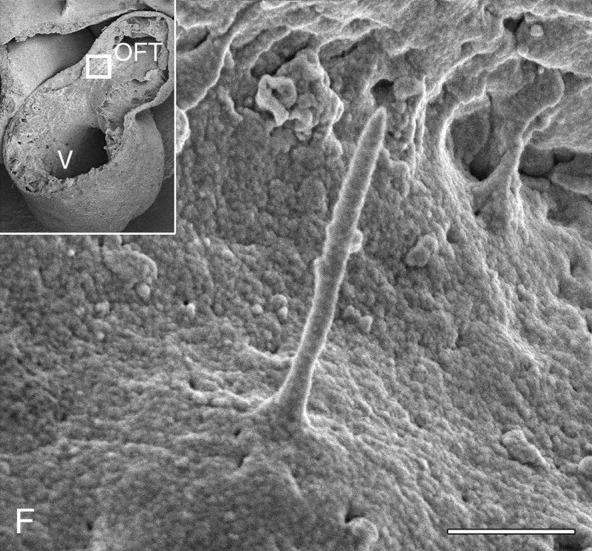
\includegraphics[width=\textwidth]{images_other/primary_cilium.jpg}%
        \caption{Primary cilium in a developing chicken heart. Image from~\citeauthor*{van_der_heiden_monocilia_2006}~\cite{van_der_heiden_monocilia_2006}. Reproduced here with permission of the copyright holder via Rightslink. © 2005 Wiley-Liss, Inc.}%
        \label{fig:sem_primary}%
    \end{subfigure}%
    \hfill
    \begin{subfigure}[t]{0.47\linewidth}%
        \centering%
        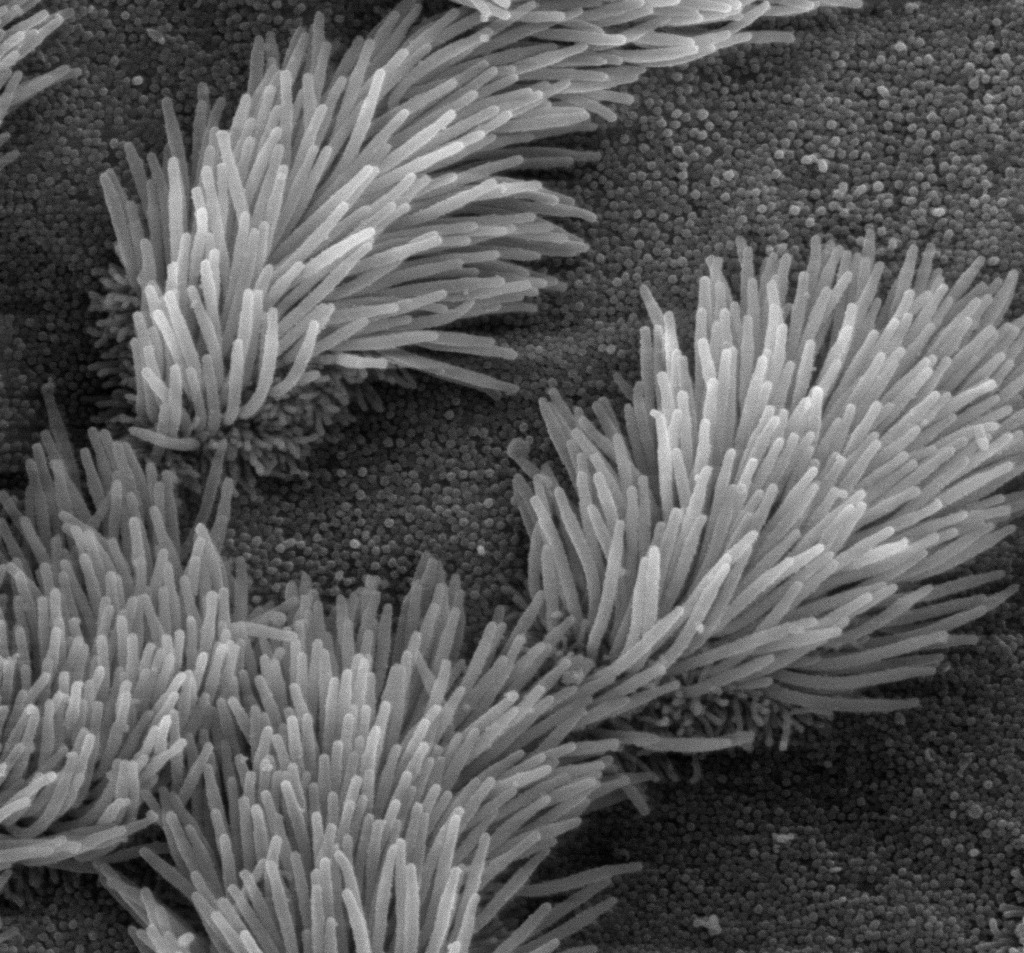
\includegraphics[width=\textwidth]{images_other/trachea_cilia_daghlian_pd.jpg}%
        \caption{Motile cilia in the human trachea. Image by Charles Daghlian and released to the public domain.}%
        \label{fig:sem_motile}%
    \end{subfigure}%
    \caption{Scanning electron microscope images of a single primary cilium (a) and bundles of motile cilia (b). The primary cilium stands alone whereas the motile cilia are found in bundles, which is typical for the two types.}%
    \label{fig:sem_photos}%
\end{figure}

Motile cilia, on the other hand, mostly have roles in fluid pumping, though recent research has also revealed that they have sensory capacity as well~\sidecite{bloodgood_sensory_2010}; this revelation is examined in much more detail in Ch.~\ref{ch:results_particle}. They are usually found in `bundles' or `carpets', where one cells hosts many cilia (imaged in Fig~\ref{fig:sem_motile}); for example, in the lungs, multiciliated cells have around 200 cilia per cell~\sidecite{horani_advances_2018}. They are also found in many places in the body: as previously mentioned, they are found in the lungs and trachea~\sidecite[-30pt]{yaghi_airway_2016}, where their waving works to move mucus out of the lungs to remove trapped pathogens and particulates. They are also found pumping fluid in the brain to move signalling molecules~\sidecite[-60pt]{olstad_ciliary_2019}, in the reproductive system (both male~\sidecite[-43pt]{yuan_motile_2019} and female~\sidecite[-5pt]{lyons_reproductive_2006}) and on the surface of microscopic organisms where they help with feeding and swimming~\sidecite{funfak_paramecium_2015, mannan_minimal_2020}. As with primary cilia, defective motile cilia lead to a large number of diseases~\sidecite{afzelius_cilia-related_2004}.

The beat of a motile cilium is asymmetric and irreversible, meaning that the problem posed by scallop theorem is avoided. The beat begins with a straightened cilium performing a power stroke, intended to move as much fluid as possible as fast as possible. The cilium then curls up and returns to its original position in a so-called recovery stroke, staying as close to the cell surface as possible~\sidecite{gueron_energetic_1999}. Due to the curled-up shape of the recovery stroke, and the no-slip condition on the cell surface, the cilium doesn't move much fluid during the recovery stroke compared to the amount moved during the power stroke, giving a net pumping effect. This beating pattern is illustrated in Fig.~\ref{fig:motile_beat}. At sufficient density, motile cilia can coordinate their beating to improve their efficiency and minimise intercilium collisions~\sidecite{osterman_finding_2011, ringers_novel_2023}; the mechanisms underpinning this behaviour are examined in Ch.~\ref{ch:results_sync}.

\begin{figure}
    \centering
    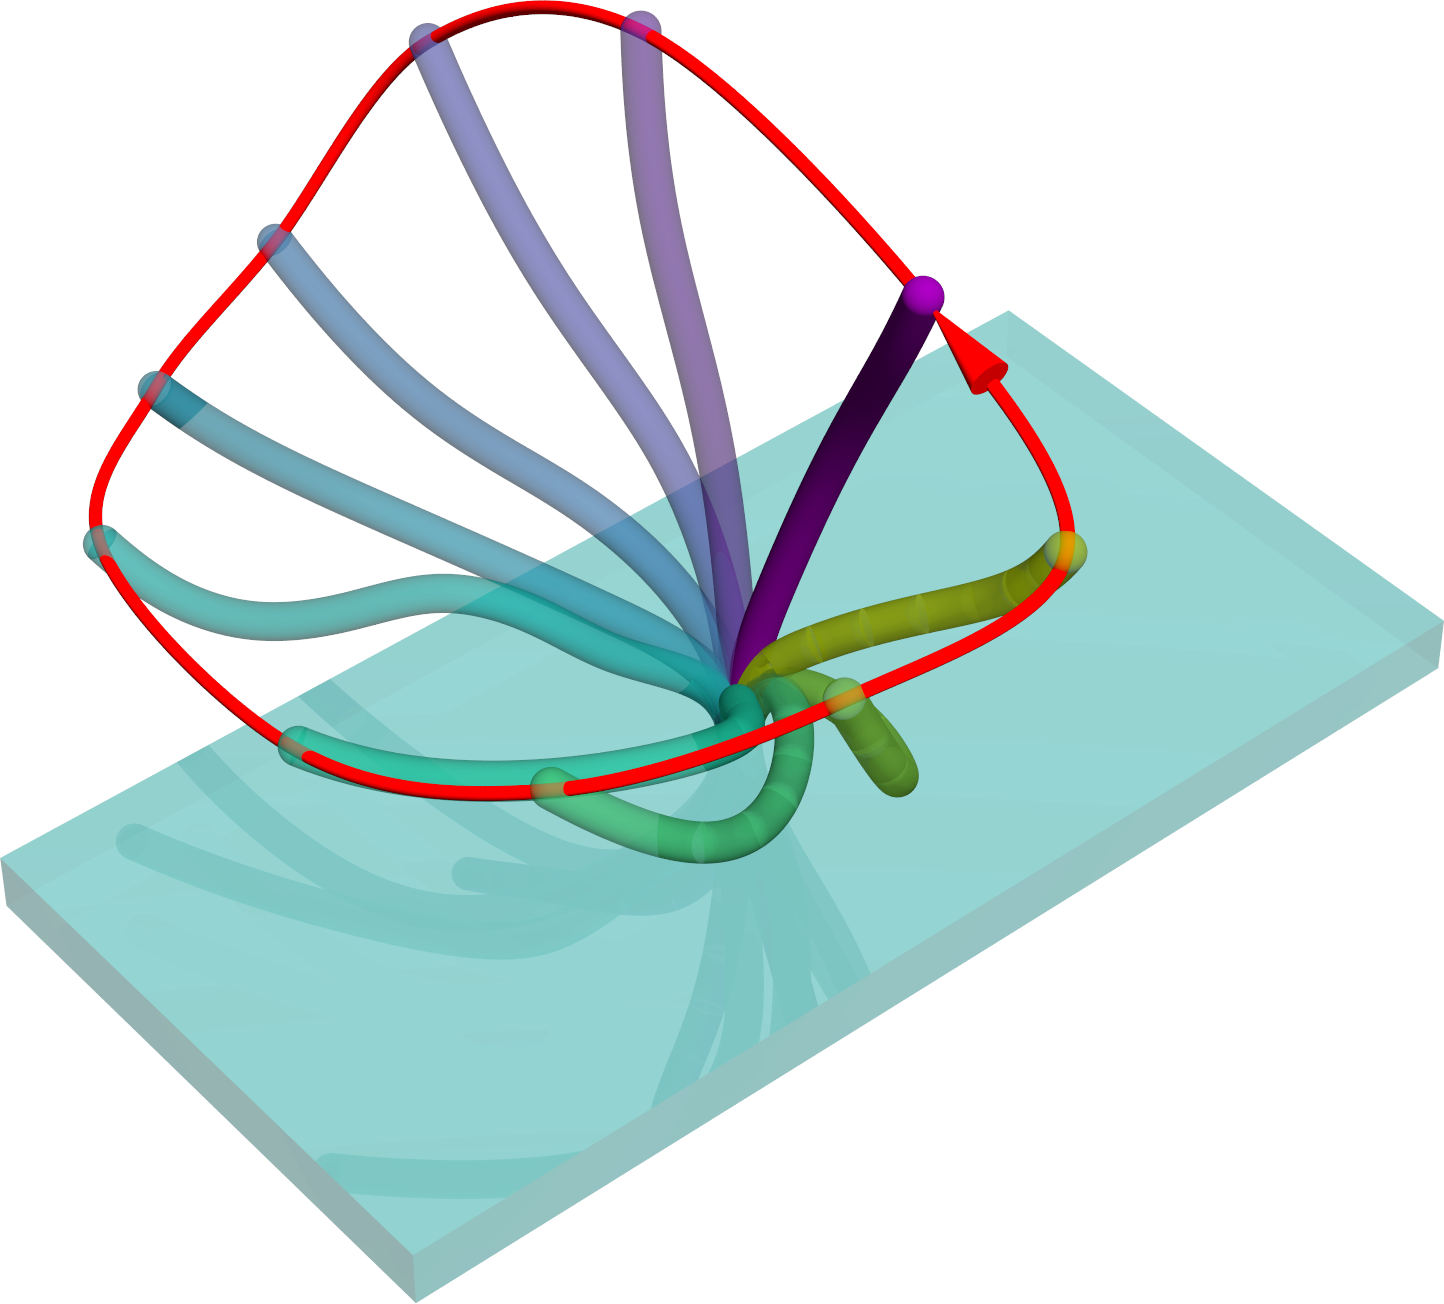
\includegraphics[width=0.6\linewidth]{images_other/enhanced_motilebeat.png}
    \caption{Motile cilium beat. The cilium performs a power stroke (solid dark blue colour), then curls up and pulls back along the cell surface. The trajectory breaks time reversal symmetry, so it can produce a net flow without falling afoul of scallop theorem.}
    \label{fig:motile_beat}
\end{figure}

Both primary and motile cilia consist of a basal body affixed to the cell, and a protruding structure with a microtubule skeleton, all covered in cell membrane. The basal body works to organise and support the microtubules. The microtubule `skeleton' of the cilium is called the axoneme, and consists of a series of nine microtubule doublets, shown in Fig.~\ref{fig:axoneme}a-b for the two cilium types. The primary cilium and the motile cilium have slightly different axonemes: the motile cilium has an additional pair of microtubules in the centre (hence the name 9+2 axoneme, for the nine outer doublets and the two inner microtubules), and some radial spokes that connect it to the outer doublets, along with some dynein arms that are responsible for sliding the microtubules relative to one another to generate bending~\sidecite{falk_specialized_2015}. The primary cilium lacks the central pair of microtubules, leading to it being named a 9+0 axoneme, as well as lacking the dynein arms and radial stokes. The structure of the motile cilium, including the additional apparatus required for motility, is shown in cross-section in Fig.~\ref{fig:axoneme_motile_2d}.

There are, however, exceptions to this seemingly neat classification: in the structure responsible for the left-right differentiation of mammalian embryos (creatively named the left-right organiser), specialised motile cilia (called `nodal cilia') lack the central pair, and they have a very different (and simpler) beating pattern compared to regular motile cilia. Kinocilia, found in the inner ear, have a 9+2 axoneme, like motile cilia, but they don't have the dynein arms and they don't move under their own power; they simply bend under the influence of external vibrations, and are usually considered to be a variant of primary cilia. There can therefore be said to be four types of cilia depending on the combination of axoneme type and motility~\cite{falk_specialized_2015}.

\begin{figure*}
    \begin{subfigure}[t]{0.49\linewidth}
        \centering
        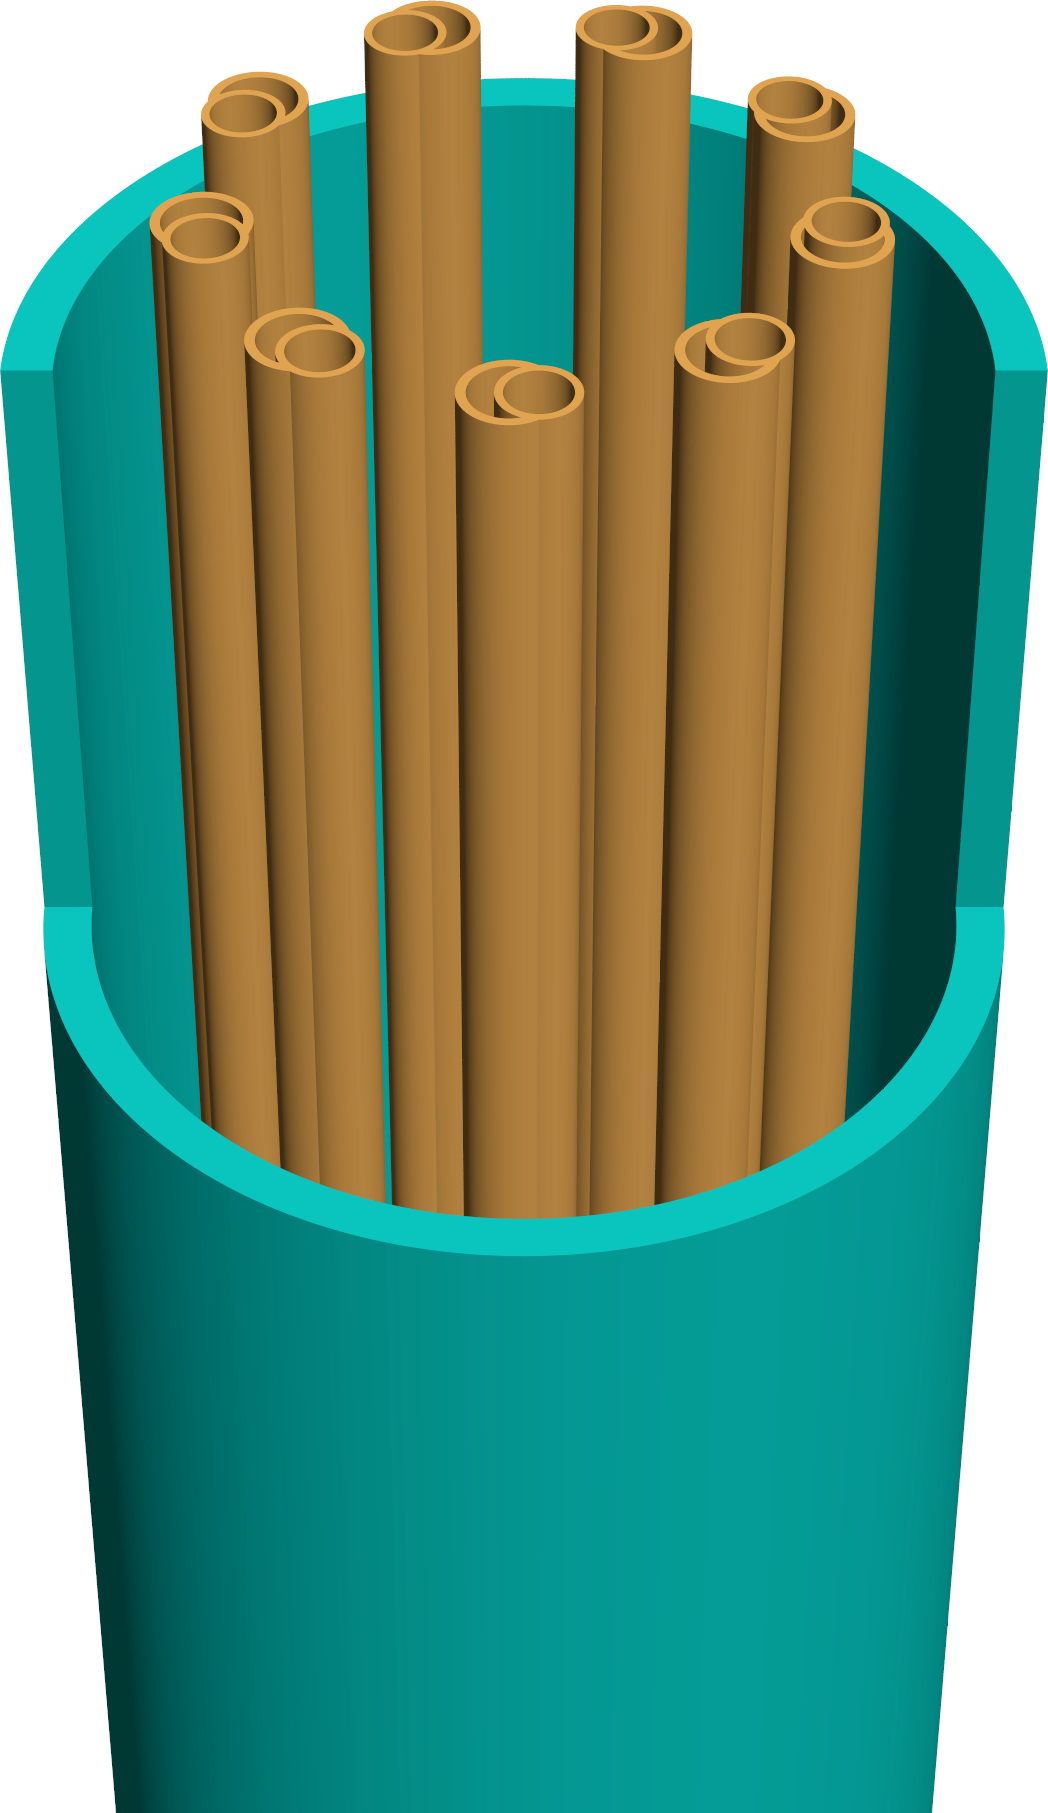
\includegraphics[width=0.50\textwidth]{images_other/enhanced_axoneme.png}
        \caption{Render of the microtubule structure of a primary cilium. Because it has nine doublets and no central pair, this arrangement is often referred to as a 9+0 axoneme.}
        \label{fig:axoneme_primary}
    \end{subfigure}
    ~
    \begin{subfigure}[t]{0.49\linewidth}
        \centering
        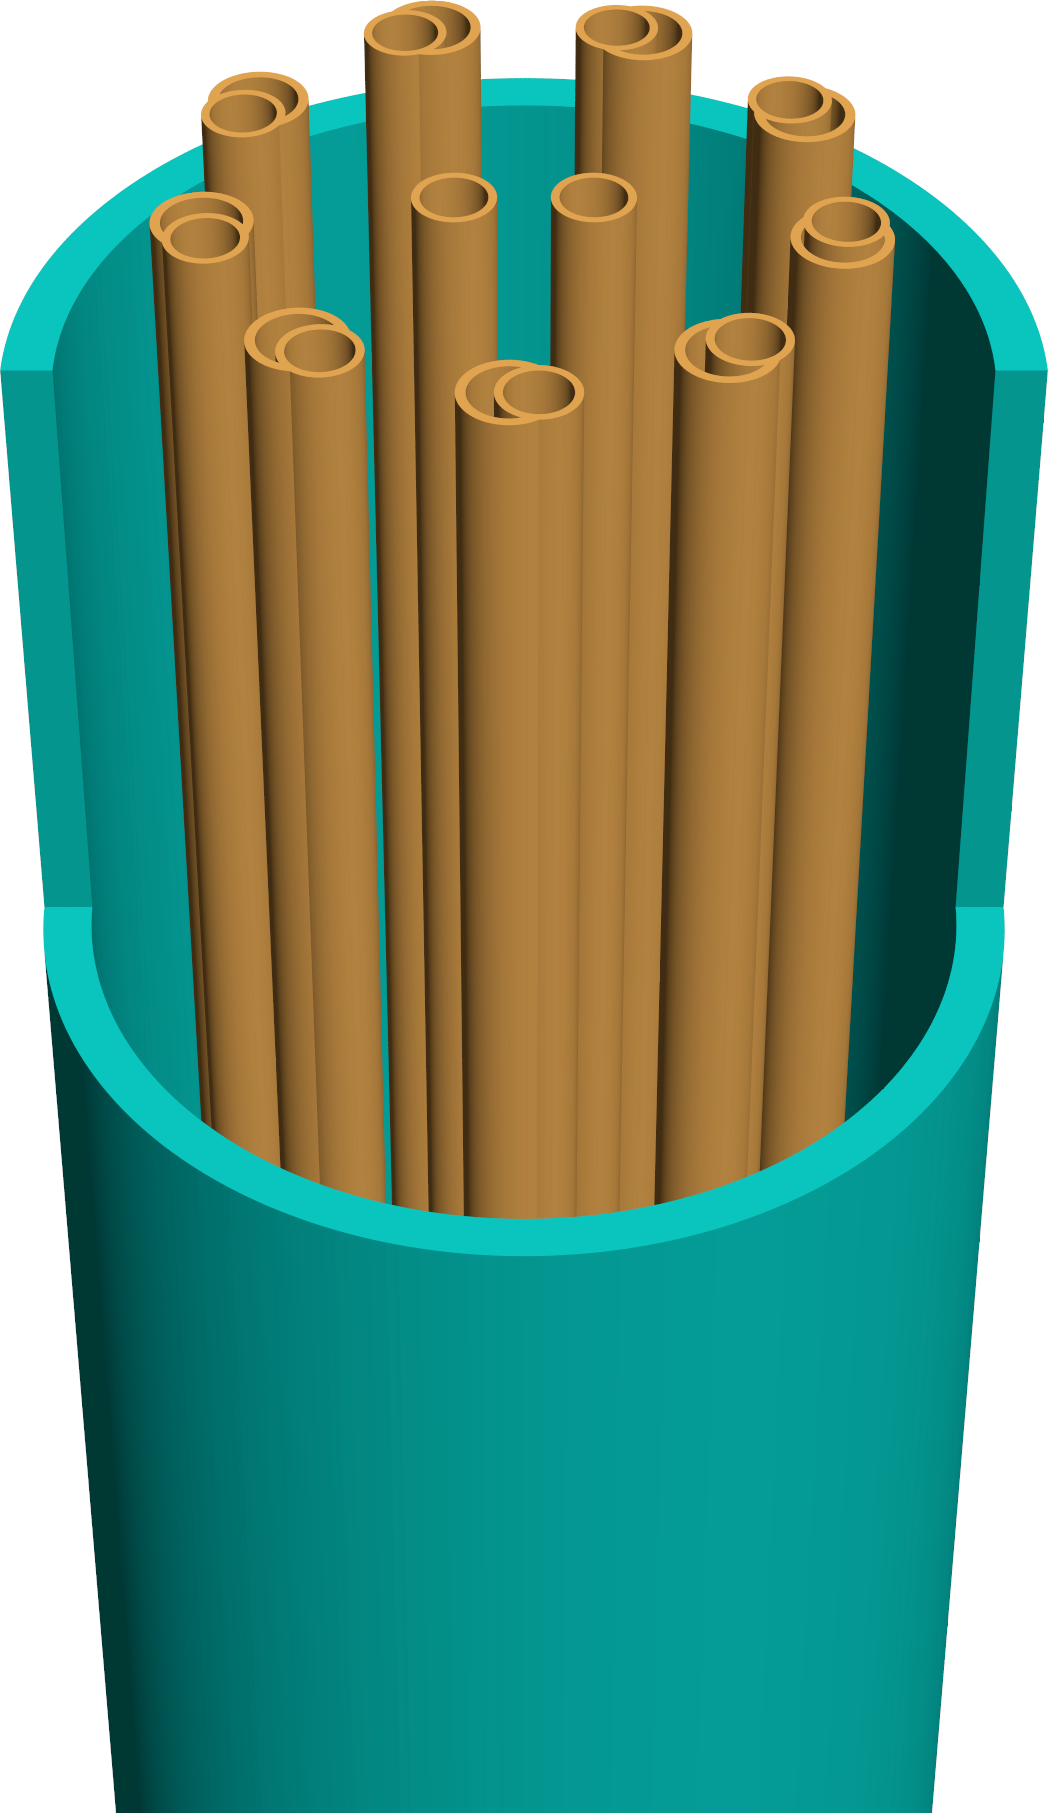
\includegraphics[width=0.50\textwidth]{images_other/enhanced_axoneme_motile.png}
        \caption{Render of the microtubule structure of a motile cilium; note the two central microtubules (which are absent in the primary cilium case) which along with the nine doublets give this axoneme arrangement its designation as a 9+2 axoneme.}
        \label{fig:axoneme_motile}
    \end{subfigure}
    
    \begin{subfigure}[t]{0.49\linewidth}
        \centering
        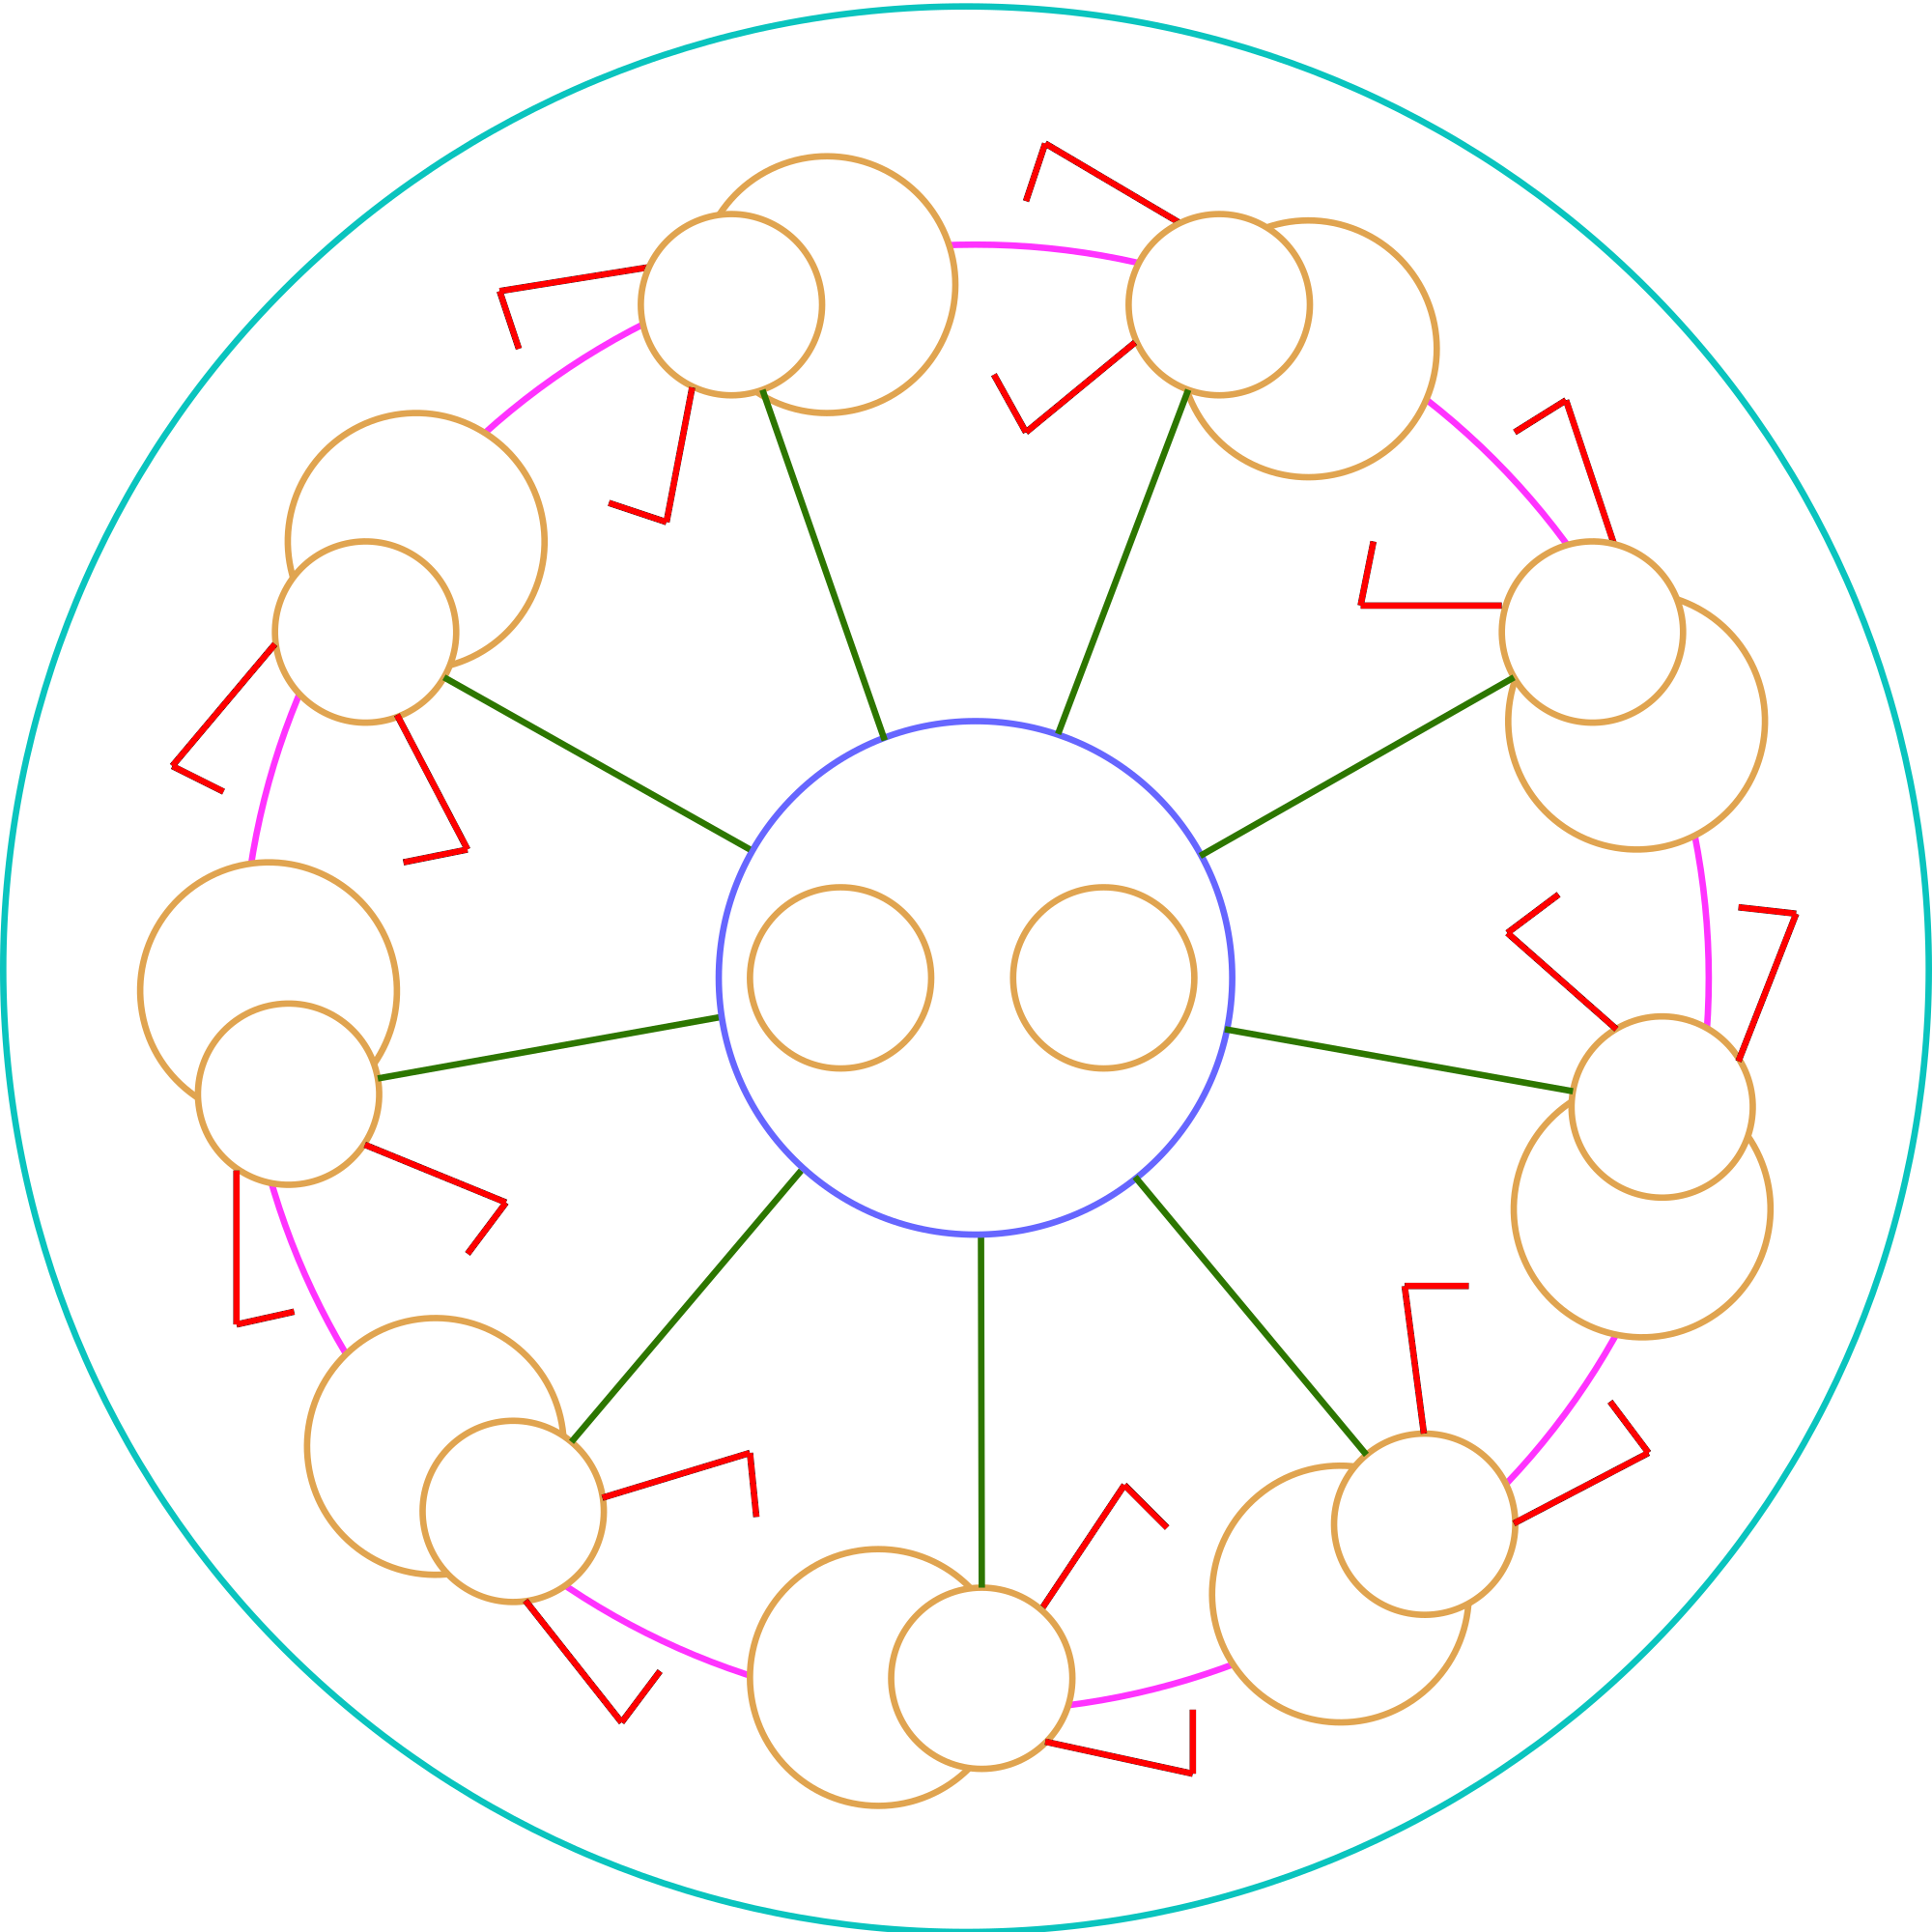
\includegraphics[width=0.8\textwidth]{images_other/axoneme_2d.png}
        \caption{Top-down view of motile cilium axoneme. The outer tubule doublets and central microtubules (yellow) are visible, along with the spokes connecting them. The dynein arms that give rise to the motility of the cilium are shown in red; these generate sliding motion between the doublets and thus create the cilium's bending motion. The primary cilium lacks almost all of the structure shown in this diagram, except for the outer doublets.}
        \label{fig:axoneme_motile_2d}
    \end{subfigure}
    ~
    \begin{subfigure}[t]{0.49\linewidth}
        \centering
        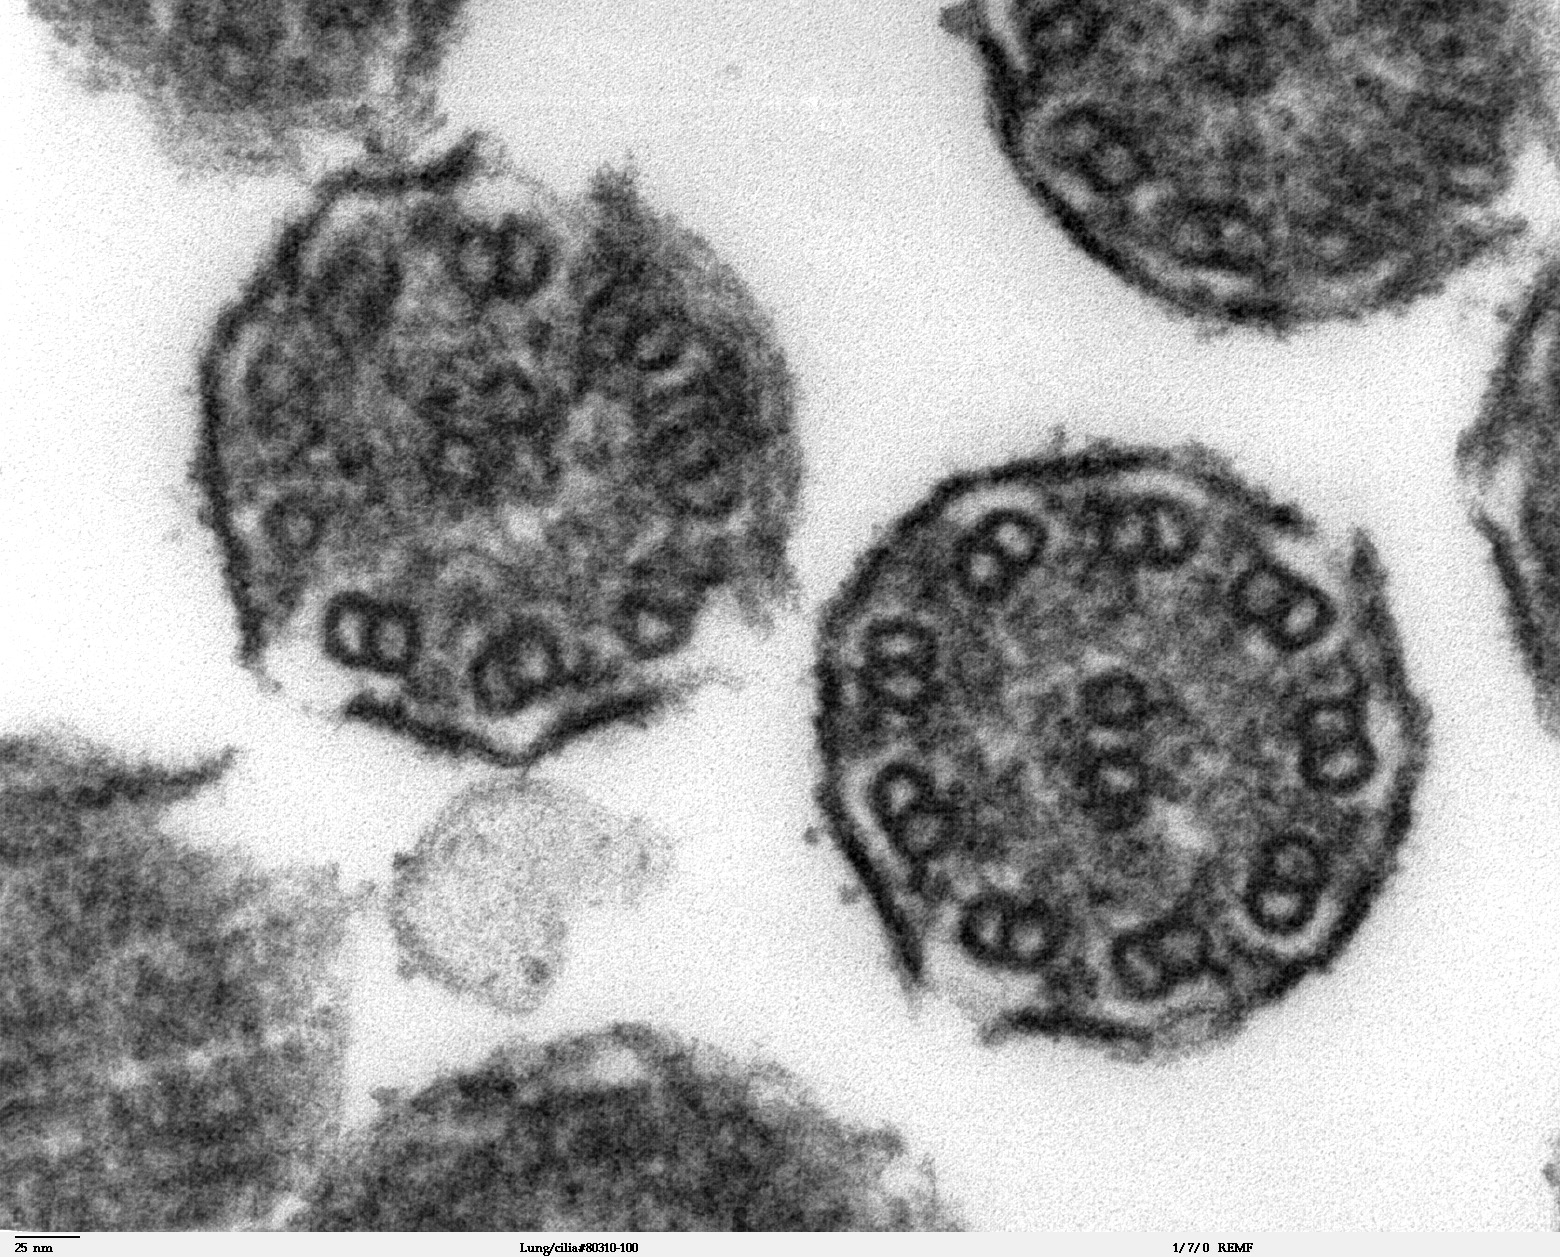
\includegraphics[width=0.9\textwidth]{images_other/lung_cilia_crosssection_howard_pd.jpg}
        \caption{Photo showing the axoneme of some motile cilia in the mammalian lung from above. The doublets are clearly visible, as is the central microtubule pair. Taken by Louisa Howard and released to the public domain.}
        \label{fig:axoneme_sem}
    \end{subfigure}
    
    \caption{Structure of the two types of cilia.}
    \label{fig:axoneme}
\end{figure*}

\section{Chapter summary}

\begin{itemize}
    \item At the length scale of cilia, fluid behaviour is dominated by viscosity, which greatly simplifies the equations of fluid motion.
    \item These simplified equations can be solved using various mobility tensors, the most relevant of which is the Rotne-Prager tensor. This approach results in high computational efficiency, even when accounting for no-slip boundaries on the surfaces of spherical bodies, or including planar no-slip boundaries.
    \item The linearity of the Stokes flow permits a lot of approaches to modelling slender bodies, and we favour an approach based on superposing Green's function solutions.
    \item Cilia come in two main types: primary and motile cilia. Both can be chemosensitive but only the motile cilia have roles in pumping.
    \item Motile cilia break time-reversal symmetry with an asymmetric beat consisting of a power and recovery stroke.
\end{itemize}

% Still TODO for this chapter:
% - explicit far field expression for Blake.
